\providecommand{\main}{..}
\documentclass[\main/main.tex]{subfiles}
\begin{document}
\chapter{Algoritmo di Dijkstra}
\section{Utilità}
L'algoritmo di Dijkstra viene utilizzato per trovare il cammino più breve tra due nodi di un grafo.
\section{Complessità}
\begin{complexity}[Algoritmo di Dijkstra]
  L'implementazione dell'algoritmo di Dijkstra iniziale ha complessità \(\O{\abs{2}^2}\).
\end{complexity}

\section{Il funzionamento di Dijkstra}
\begin{enumerate}
  \item Inizialmente tutti i nodi sono marcati come \textbf{non visitati} e viene assegnata ad ognuno di essi un valore di distanza: \(0\) per il nodo iniziale ed \(\infty \) per tutti gli altri.
  \item Per il nodo corrente, prendiamo in considerazione tutti i nodi vicini non visitati: per ognuno calcoliamo la distanza dalla radice passando attraverso il nodo corrente e confrontiamo il valore di distanza preesistente con quello nuovo e manteniamo il valore minore.\label{Dijkstra_first}
  \item Una volta determinata la distanza per tutti i vicini del nodo corrente marchiamo il nodo corrente come \textbf{visitato}.
  \item Se il \textbf{nodo destinazione} è stato marcato visitato o se la lunghezza minore tra i nodi non visitati è infinita (come quando si vuole raggiungere un nodo non connesso) l'algoritmo si interrompe.
  \item Altrimenti si sceglie un nodo non visitato a distanza minima: esso diviene il nuovo nodo corrente e l'operazione si ripete dal punto \ref{Dijkstra_first}.
\end{enumerate}
\clearpage
\section{Step by step}
\begin{figure}
  \begin{subfigure}{0.49\textwidth}
    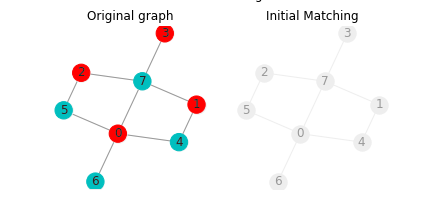
\includegraphics[width=\textwidth]{dijkstra/0}
  \end{subfigure}
  \begin{subfigure}{0.49\textwidth}
    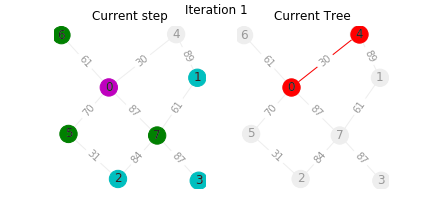
\includegraphics[width=\textwidth]{dijkstra/1}
  \end{subfigure}
  \begin{subfigure}{0.49\textwidth}
    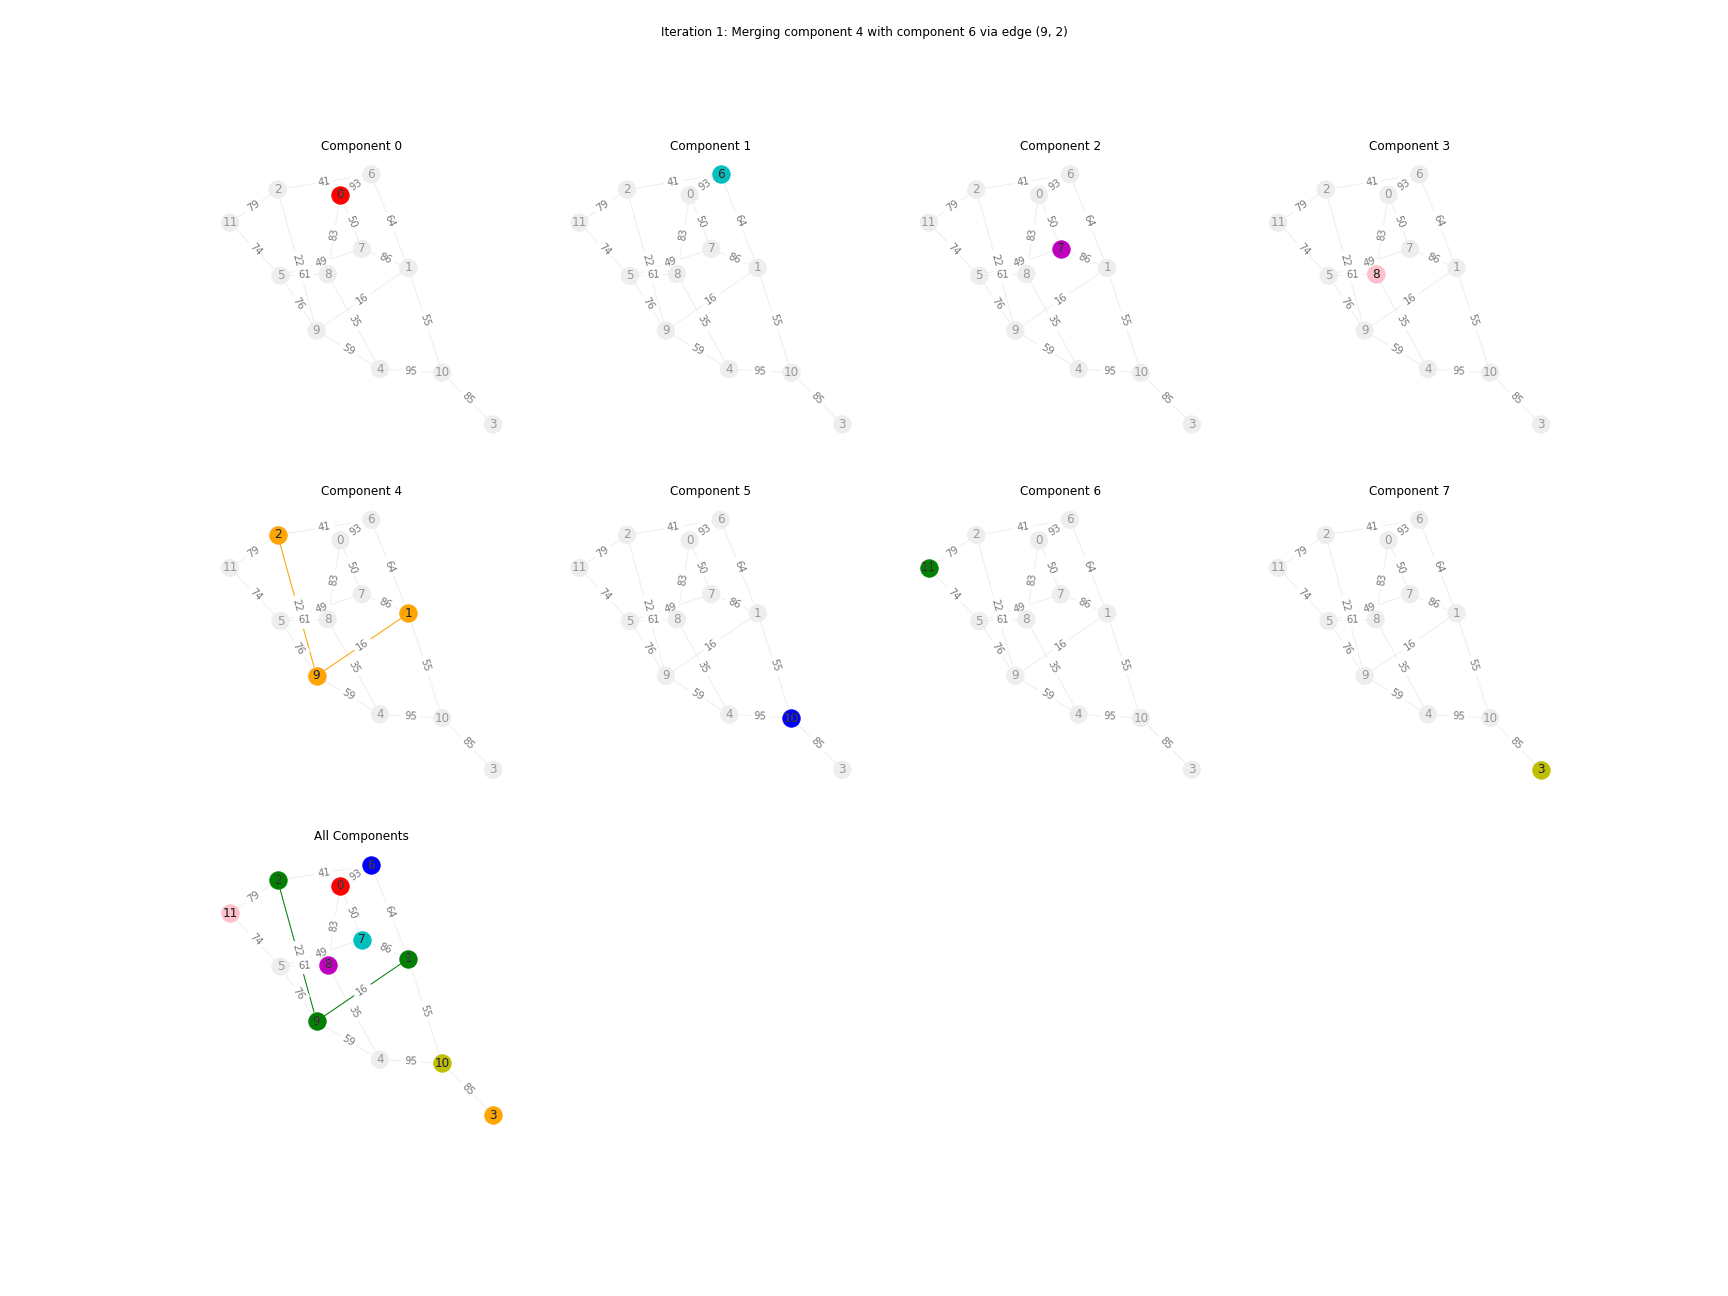
\includegraphics[width=\textwidth]{dijkstra/2}
  \end{subfigure}
  \begin{subfigure}{0.49\textwidth}
    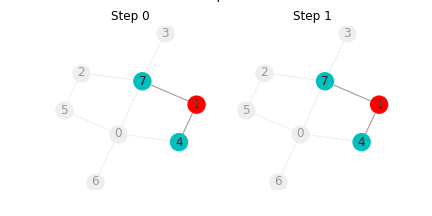
\includegraphics[width=\textwidth]{dijkstra/3}
  \end{subfigure}
  \begin{subfigure}{0.49\textwidth}
    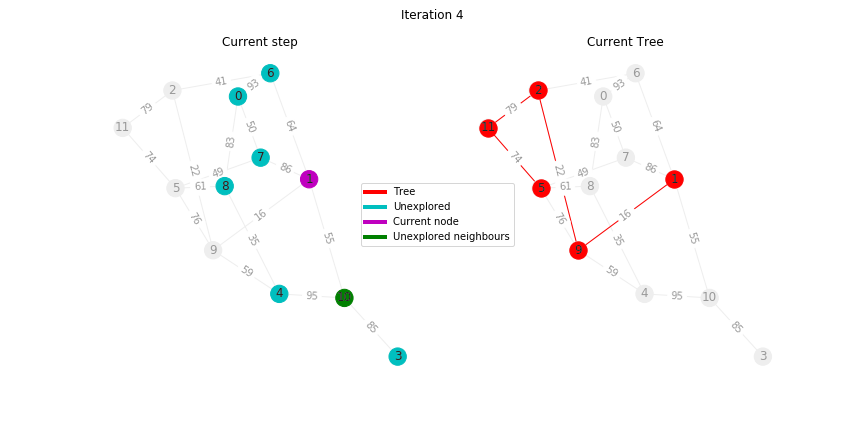
\includegraphics[width=\textwidth]{dijkstra/4}
  \end{subfigure}
  \begin{subfigure}{0.49\textwidth}
    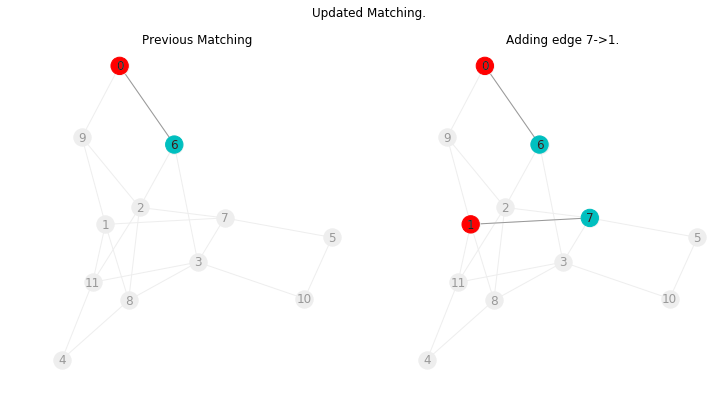
\includegraphics[width=\textwidth]{dijkstra/5}
  \end{subfigure}
  \begin{subfigure}{0.49\textwidth}
    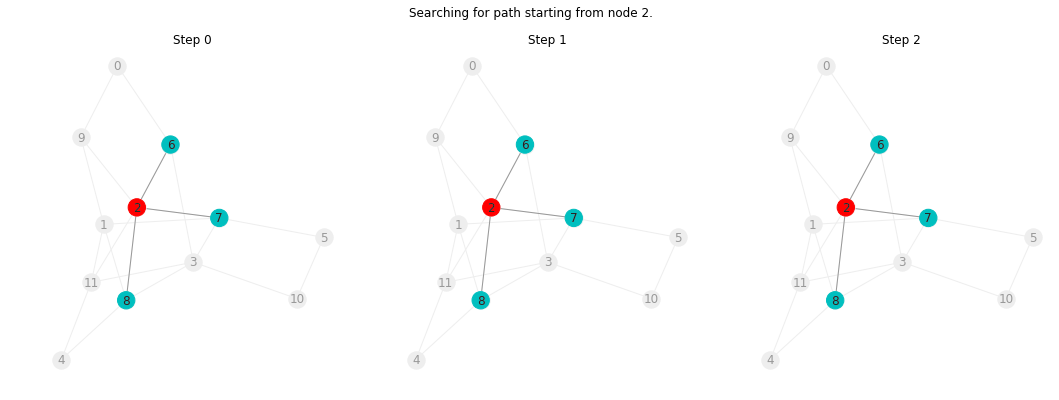
\includegraphics[width=\textwidth]{dijkstra/6}
  \end{subfigure}
  \begin{subfigure}{0.49\textwidth}
    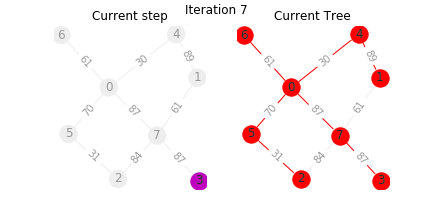
\includegraphics[width=\textwidth]{dijkstra/7}
  \end{subfigure}
  \begin{subfigure}{0.25\textwidth}
    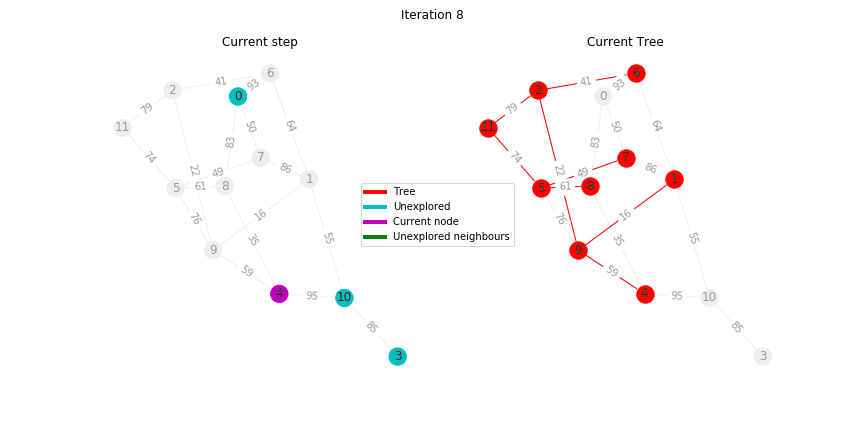
\includegraphics[width=\textwidth]{dijkstra/8}
  \end{subfigure}
\end{figure}


\clearpage
\section{Correttezza di Dijkstra}
\begin{proof}[Correttezza di Dijkstra]
  Procediamo a dimostrare la correttezza dell'algoritmo di Dijkstra \textbf{per induzione} sul numero di nodi visitati.

  Per ogni nodo visitato \(v\), la distanza \(d(v)\) è la distanza minore dal nodo sorgente al nodo \(v\). Per ogni non non visitato \(u\), \(d(u)\) è assunta essere la distanza più breve attraverso solo nodi visitati, dalla radice a \(u\).

  Questa assunzione vale solo se un cammino esiste, altrimenti la distanza è inizializzata a \(\infty \).

  Il caso base è quando esiste solo un nodo visitato, cioè il nodo sorgente, in tal caso l'ipotesi è banale.

  Altrimenti, assumiamo l'ipotesi per \(n-1\) nodi visitati. In tal caso, scegliamo un lato \(\rnd{v,u}\) dove \(u\) possiede la distanza minima di ogni nodo non visitato ed il lato \(\rnd{v,u}\) è tale che:
  \[
    d(u) = d(v) + \text{lunghezza}(v, u)
  \]
  La distanza \(d(u)\) è considerata la distanza minore dalla \textbf{radice} a \(u\) perché se esistesse un cammino più breve e se \(w\) fosse il primo nodo non visitato su quel cammino allora l'ipotesi originale che \(d(w) > d(u)\) \textbf{non sarebbe più valida}.

  Similarmente se vi fosse un cammino più breve per giungere ad \(u\) senza utilizzare nodi non visitati e se il penultimo nodo su questo cammino fosse \(w\), allora si avrebbe che \(d(u) = d(w) + \text{lunghezza}(w, u)\) \textbf{che è nuovamente una contraddizione}.

  Dopo aver processato il nodo \(u\), le ipotesi iniziali si manterranno vere per ogni non visitato \(w\): la distanza \(d(w)\) sarà la distanza minore dalla radice a \(w\) utilizzando solo i nodi visitati perché se esistesse un cammino più breve non passante per \(u\) lo avremmo identificato precedentemente, e se esistesse un cammino più breve passante passante per \(u\) lo avremmo aggiornato mentre il nodo \(u\) veniva processato.
\end{proof}
\clearpage
\subsection{Diagramma della dimostrazione - Correttezza di Dijkstra}
\begin{figure}
  \includegraphics[width=0.7\textwidth]{proofs/Dijkstra}
\end{figure}
\end{document}